\documentclass{article}
\usepackage[utf8]{inputenc}

\title{Fingers}
\author{damiano.tomaino }
\date{October 2018}


\usepackage{natbib}
\usepackage{graphicx}
\usepackage{wrapfig} %add picture with text all around
\usepackage{subcaption} %for the subpictures

\begin{document}


\maketitle

\section{Introduction}

We decided to add actuators to the gripper to improve his performance. The idea was to combine the jamming with hydrostat actuators with a geometry made to have a flexible internal volume that allows the structure to bend like a finger, helping the gripper to take objects of differing shapes and sizes.

\begin{wrapfigure}{h}{0.25\textwidth}
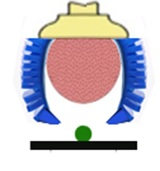
\includegraphics[scale=0.7]{Pictures/first_idea.jpg}
\caption{The first conceptual design}
\label{fig:firstIdea}
\end{wrapfigure} 

We decided to start with the simplest design possible with the actuators attached to the outside of the membrane as represented on the right. In that way we don’t have to change the actual design and the test phase will be fast.
The actuators have the only task of better distributing the unjammed particles around the object, while membrane must still maintain a strong hold. The material of the actuators must be soft to avoid damages on the objects. 
There are many projects about actuators in soft robotics. One way to realize them found in literature [1] is using a mold 3D printed to create fingers in silicone rubber. The shape of the mold was based on this one, with some changes to easily connect it to our gripper.

\begin{figure}[h]
 
\begin{subfigure}{0.5\textwidth}
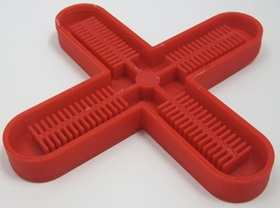
\includegraphics[width=0.8\linewidth, height=4cm]{Pictures/moldFromTutorial.jpg} 
\caption{Picture extracted from the tutorial}
\label{fig:moldTut}
\end{subfigure}
\begin{subfigure}{0.5\textwidth}
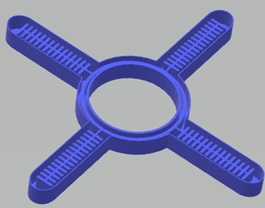
\includegraphics[width=0.8\linewidth, height=4cm]{Pictures/OurFirstMold.jpg}
\caption{First mold designed}
\label{fig:subim2}
\end{subfigure}
 
\caption{Caption for this figure with two images}
\label{fig:image2}
\end{figure}

For the first test it was chosen a length of the actuators of 4 inches and a width of 1 inch. 
As shown on the pictures there are many chambers in the actuator and air pumped in the 4 actuators will bend them. 
The mold was printed in PLA with the 3D printer model \textbf{Prusa I3 MK2S} and for the actuators the material chosen was \textbf{\textit{Ecoflex 00-30 [1]}}, bought on \underline{www.reynoldsam.com}. This material is a silicone rubber extraordinarily soft, strong and durable.

As described on Instructables \cite{Air-Powered Soft Robot Gripper}, the separate fingers were closed by a bigger layer of silicon rubber.

\begin{figure} [h]
    \centering
    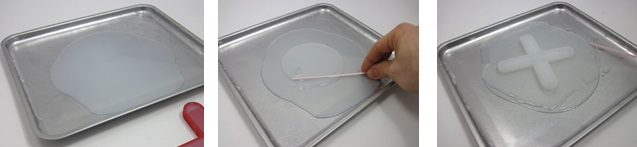
\includegraphics[width=1\textwidth]{Pictures/StepCloseFingers.jpg}
    \caption{picture from the tutorial to close ecoflex}
    \label{fig:tutorialProcess}
\end{figure}

\section{Results with the first geometry}

The results were not satisfactory. The mold was not right positioned and the silicon was not evenly distributed. 
\begin{figure}[h]
    \centering
    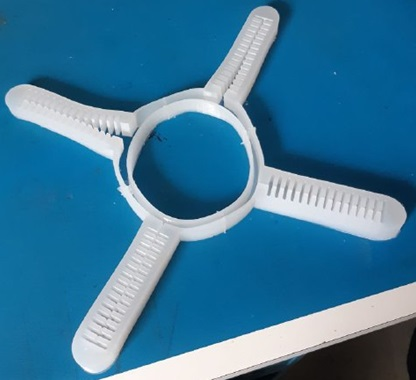
\includegraphics[scale=0.5]{Pictures/FirstResult.jpg}
    \caption{First result from the mold}
    \label{fig:firstMold}
\end{figure}

The casting was divided in four parts to test every finger separately, and to realize four different tests.
To bend in a good way, the actuator’s sides need to have two different stiffness, so that one side will stretch and the other just bend. In that way the movement of the actuator was not good controlled and the grip not strong enough. It was necessary to tighten up one side of the finger.

\section{Steps to realize the soft robotic finger}
We tried to realize a finger realized by a high repeatable process.
To do that we are using three different molds. 

PICTURE OF THE MOLDS

It is based on 6 steps:
\begin{enumerate}
\item Filling of the first mold with EcoFlex 0030
\item Add a layer of Smooth-Sil 950
\item Ribbon wrapping
\item Cover all with SortaClear 40 using the second mold
\item Realize the cover to joint the finger with the connector with the third mold
\item Use the silicone glue to attach the connector inside the cover realized
\end{enumerate}

Every time a mold is filled by a silicon rubber we used the vacuum chamber at 1 bar \emph{at about} 5 minutes, to reduce the number of bubbles, and the pressure chamber at 2 bar for all the time of curing to reduce the dimension of the bubbles remained in the mix .

PICTURES OF VACUUM CHAMBER AND PRESSURE CHAMBER


\subsection{EcoFlex 0030}
To realize the first step we used the EcoFlex 0030 in the first mold. The internal cavity is realized by a cylindrical aluminum pin of 4mm of diameter, that will be extracted after the third step.
For this step it is necessary approximately 20 grams of silicon rubber. 
To control as well as possible the quantity the mold has a line defining the boundary to reach.

PICTURE OF THE LINE IN THE FIRST MOLD


\subsection{Smooth-Sil 950}

\begin{wrapfigure}{r}{0.5\textwidth}
\centering
    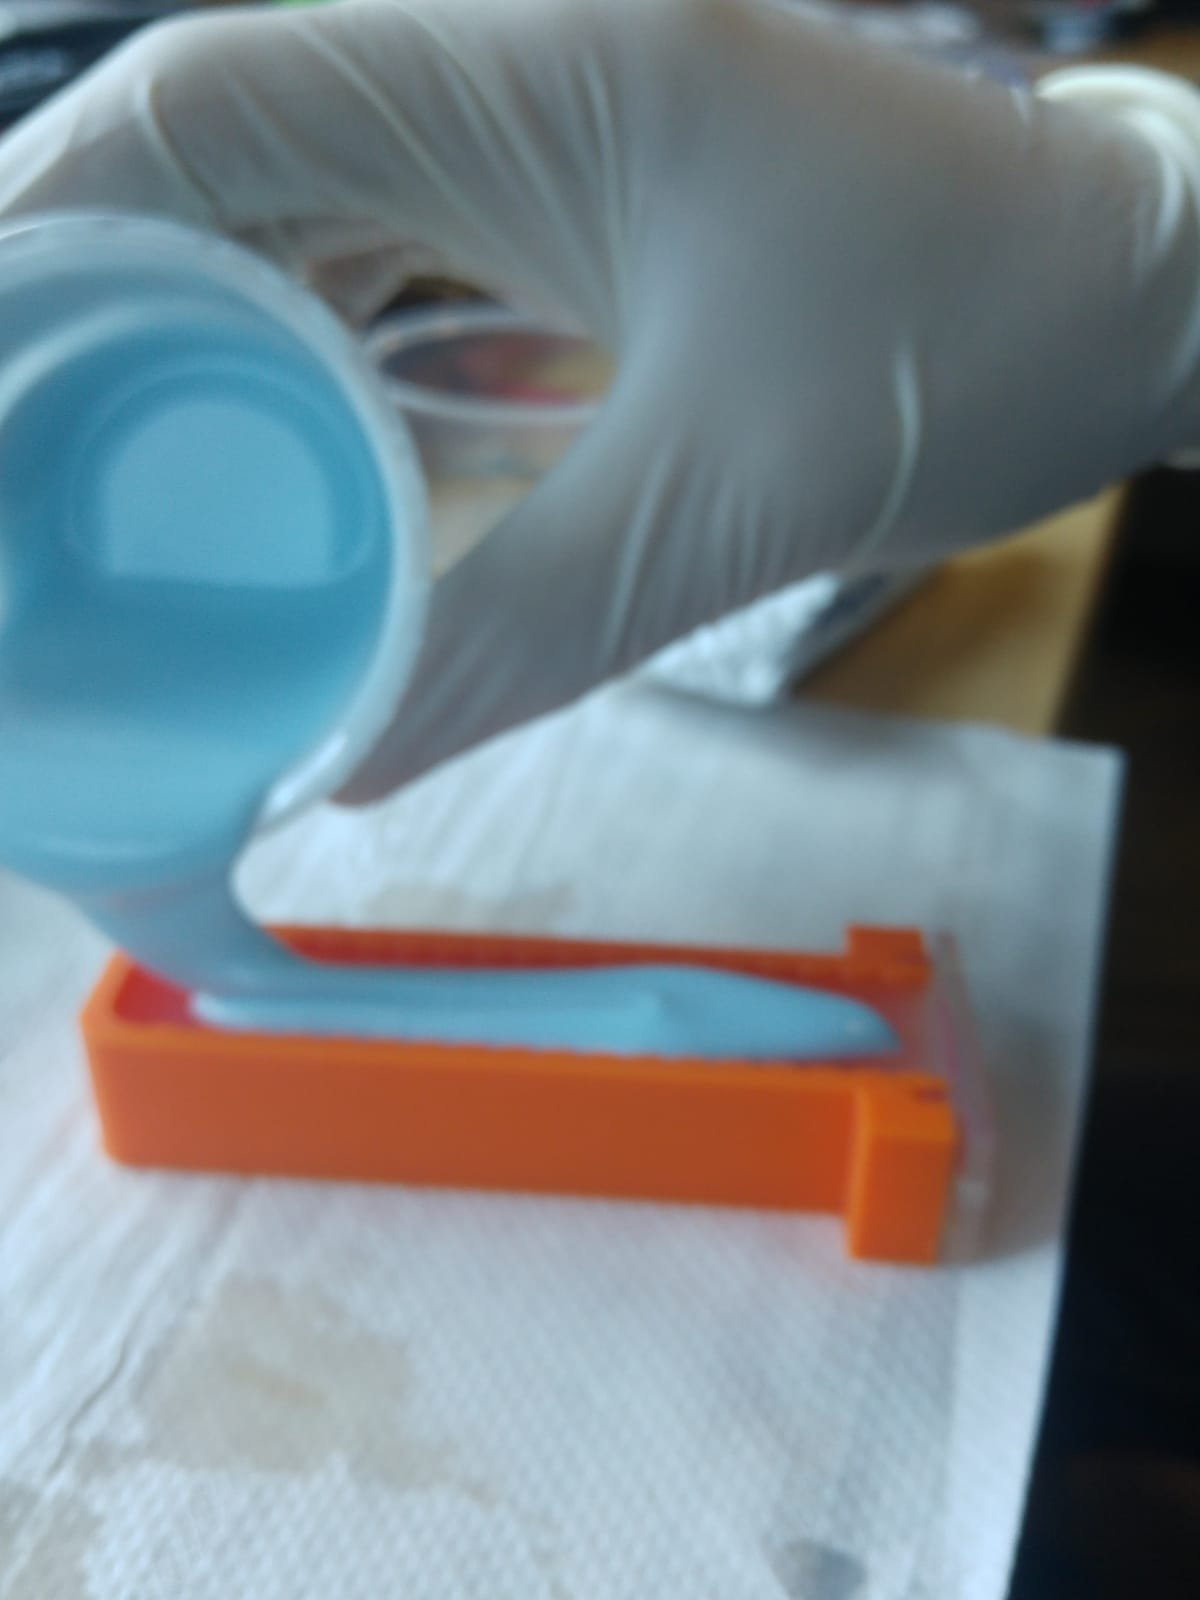
\includegraphics[width=0.25\textwidth]{Pictures/fingerOnToroidal/SmoothSil950filling.jpg}
    \caption{Smooth-Sil 950 filling}
    \label{fig:SmoothSil950filling}
\end{wrapfigure}

To bend the finger with the high pressure it is necessary a stronger layer to allow the bending, preventing the elongation in one side.
After few tests we decided to use this material. Without put out the solidified EcoFlex from the first mold it is filled the remaining space in the first mold with the Smooth-Sil 950, in that way is easily controlled the thickness of this layer.

\subsection{Ribbon wrapping}

 

\newpage

\section{Implementation of the soft fingers to the double gripper on arm in water}
Between the goal was to update and test the double gripper on arm in water.
\begin{itemize}
    \item	Replace all the hard component with soft components.
    \item	Print hydraulic manifold in water resistant material.
    \item	Refurbish water hydraulic system on arm to provide pressure and suction on different channels.
\end{itemize}

Among the components of the double gripper there were a central holding in PLA designed to have the toroidal shape and a strong cup to direct the movement of the balloon.\\
\begin{figure}[h]
    \centering
    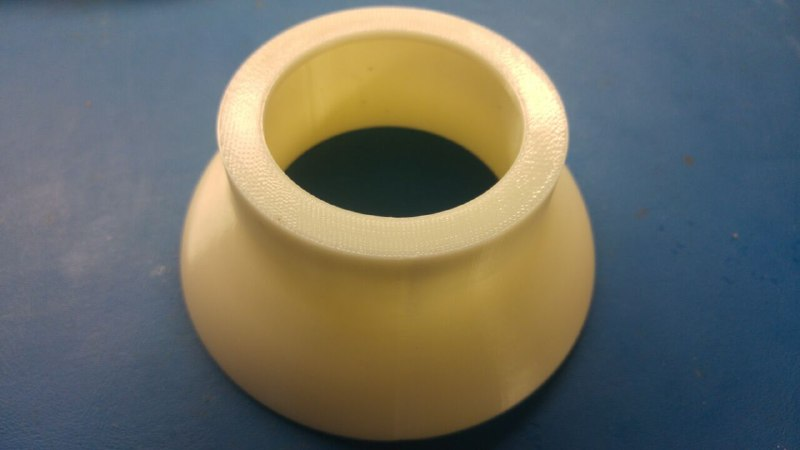
\includegraphics[width=0.4\textwidth]{Pictures/fingerOnToroidal/cup.jpg}
    \caption{Cup}
    \label{fig:cup}
\end{figure}

\begin{figure}[h]
    \centering
    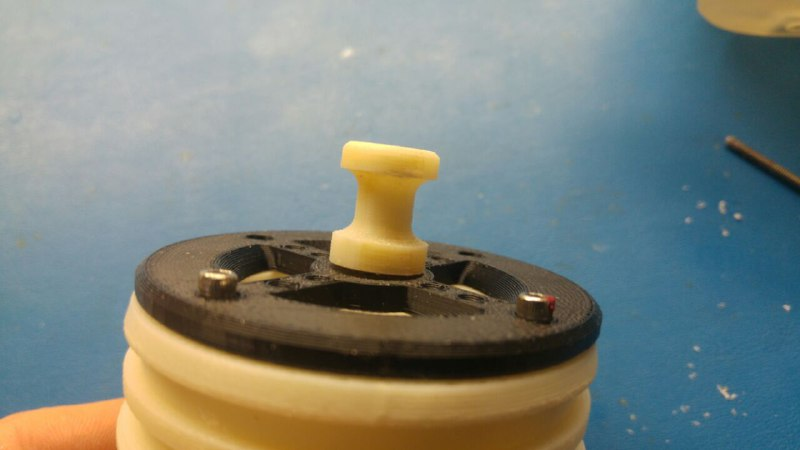
\includegraphics[width=0.4\textwidth]{Pictures/fingerOnToroidal/centralHolding.jpg}
    \caption{Central Holding}
    \label{fig:centralHolding}
\end{figure}

We chose to replace the central holding with a flexible silicone rubber tube of 5mm of diameter, the balloon will be connected on that tube by a cable tie. Therefore during the jamming also the center of the balloon is flexible and it cannot damage the object that it is grabbing.

\begin{figure}[h]
    \centering
    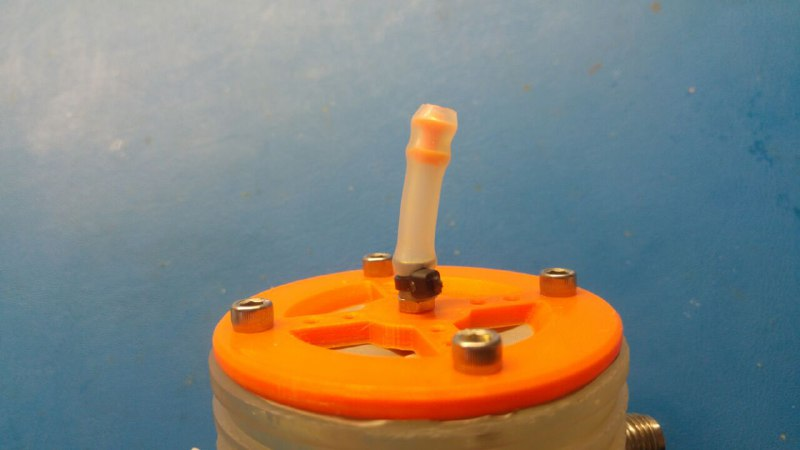
\includegraphics[width=0.4\textwidth]{Pictures/fingerOnToroidal/NewCentralHolding.jpg}
    \caption{New central holding}
    \label{fig:newCentralHolding}
\end{figure}

The cup was replaced by 3 soft hydraulic fingers. To connect the 3 fingers we designed a new manifold with a second chamber to control the pressure inside the fingers separately from the balloon.

\begin{figure}[h]
    \centering
    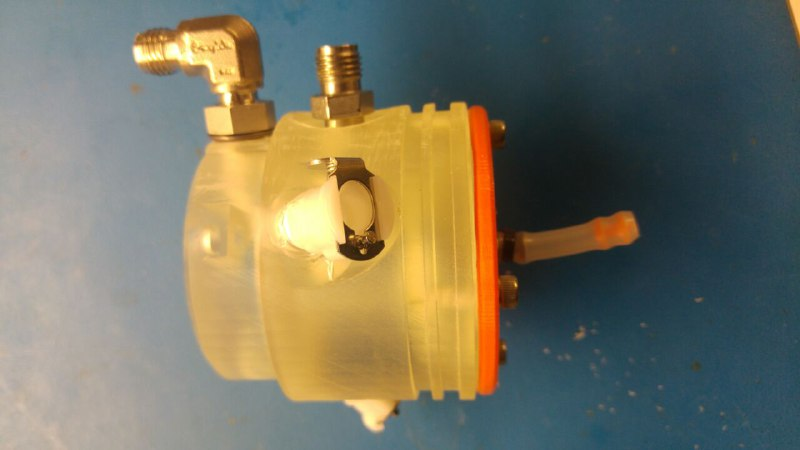
\includegraphics[width=0.4\textwidth]{Pictures/fingerOnToroidal/NewManifold.jpg}
    \caption{New manifold}
    \label{fig:newManifold}
\end{figure}

\begin{figure}[h]
    \centering
    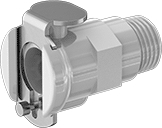
\includegraphics[width=0.25\textwidth]{Pictures/fingerOnToroidal/Plastic_quick_disconnect_tube.png}
    \caption{The quick disconnect tube (https://www.mcmaster.com/5012K29)}
    \label{fig:quickDisconnector}
\end{figure}

The manifold in the picture was printed by the 3D printer Form Lab 2 in clear resin. This is a water resistant material as requested.
The fingers are easily connected to the manifold by plastic quick-disconnect tube.

\begin{figure}[h]
    \centering
    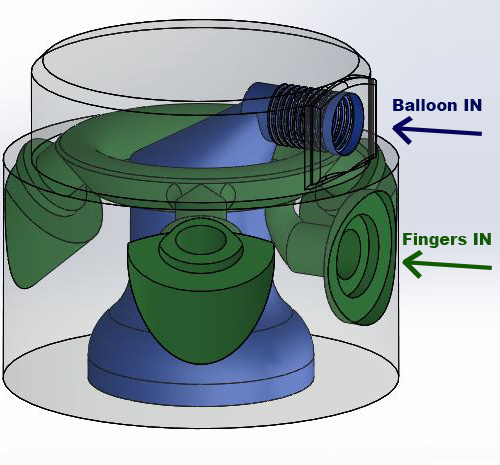
\includegraphics[width=0.8\textwidth]{Pictures/fingerOnToroidal/ManifoldSchemeFlowPhotoshop.jpg}
    \caption{Manifold flow scheme} 
    \label{fig:flowSchemeManifold}
\end{figure}



%Bibliographic references

\begin{thebibliography}
\bibitem{Air-Powered Soft Robot Gripper} https://www.instructables.com/id/Air-Powered-Soft-Robotic-Gripper/
\end{thebibliography}
\end{document}
